\textbf{Neutrinos and Neutrino Scattering}

Proof neutrinos have flavour: this doesn't happen
\begin{center}
    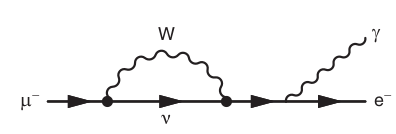
\includegraphics[width=0.3\linewidth]{images/neutrino_flavour.png}
\end{center}

Solar neutrino problem: only 1/3 of neutrinos from the sun were electron ones, should be 100\% but neutrino mixing happens.

PMNS matrix describes how neutrinos mix

\begin{center}
    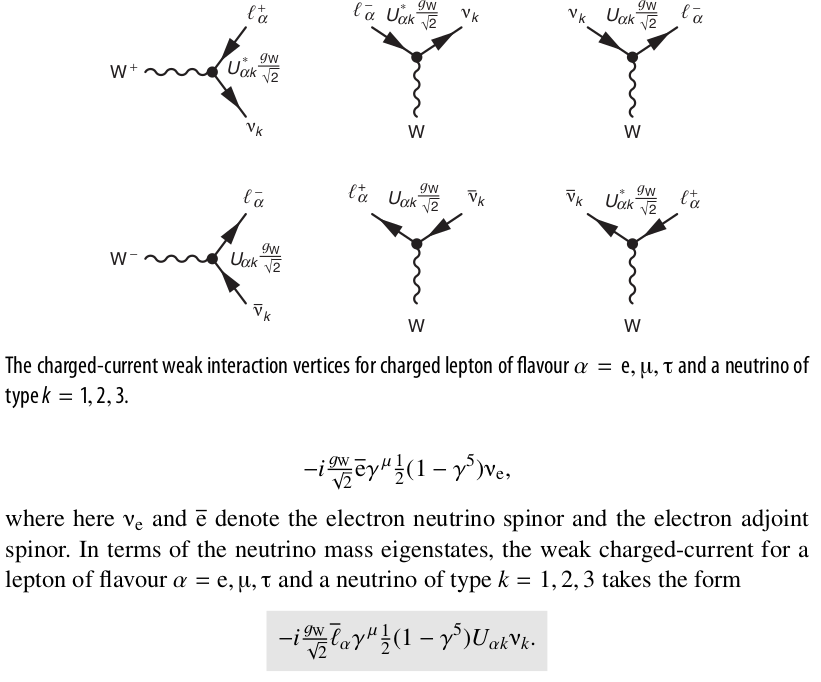
\includegraphics[width=\linewidth]{images/neutrino_production.png}
\end{center}

Studying 2-neutrino mixing can give the general idea:

Transition probability:
$P(\nu_e \to \nu_\mu) = \sin^2(2\theta) \sin^2(\frac{(m_1^2 - m_2^2) L}{4E_\nu})$

Survival probability:
$P(\nu_e \to \nu_e) = 1 - \sin^2(2\theta) \sin^2(\frac{(m_1^2 - m_2^2) L}{4E_\nu})$

\begin{center}
    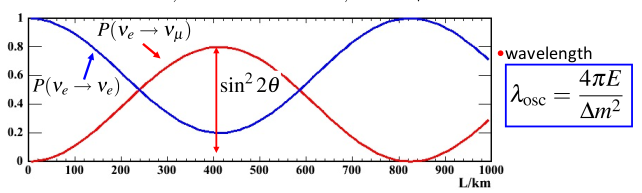
\includegraphics[width=\linewidth]{images/neutrino_oscillations.png}
\end{center}
With 3 flavours:
\begin{center}
    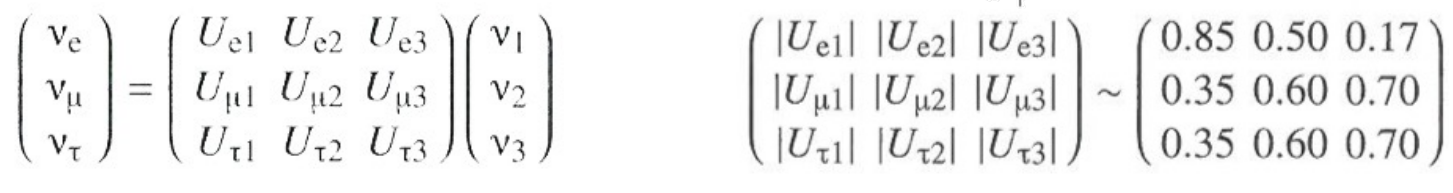
\includegraphics[width=\linewidth]{images/pmns.png}
\end{center}
An example of how to use that:
\begin{center}
    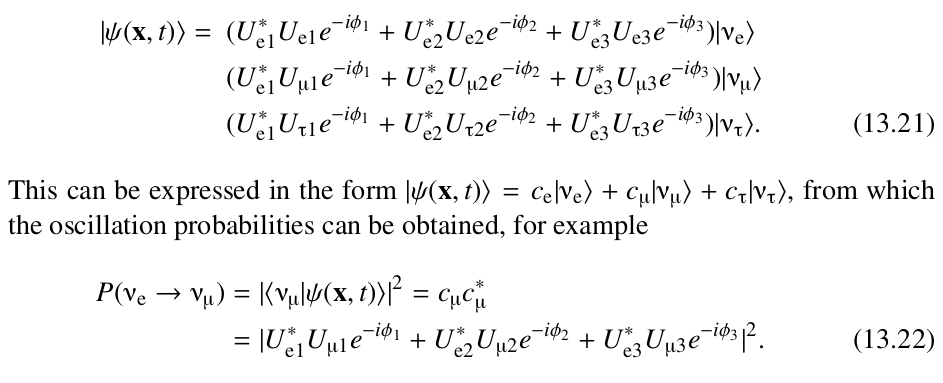
\includegraphics[width=\linewidth]{images/pmns_example.png}
\end{center}
This allows us to get mass differences but not mass hierarchy.

CP violated in weak interaction only, CPT truly conserved (SM).

One possible parametrization:
\begin{center}
    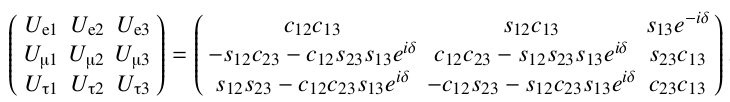
\includegraphics[width=\linewidth]{images/pmns_parametrization.png}
\end{center}

$\Delta m_{21}^2 = (7.6 \pm 0.2) \times 10^{-5} \SI{}{eV^2}$

$\sin^2(2\theta_{12}) = 0.87 \pm 0.04$

$\Delta m_{32}^2 = \SI{2.3e-3}{eV^2}$

$\theta_{12} \approx 35^\circ$, $\theta_{23} \approx 45^\circ$, $\theta_{13} \approx 10^\circ$



